Pictures are here. 
\begin{figure}
    \centering
    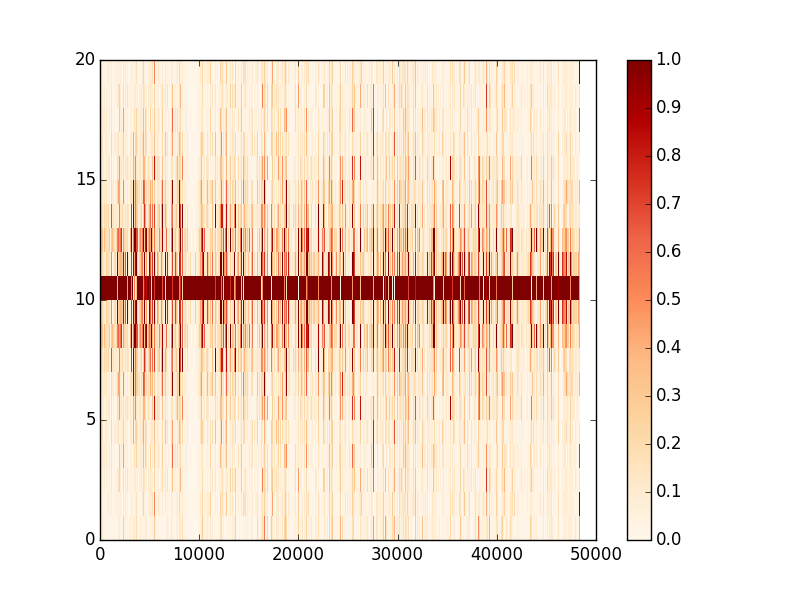
\includegraphics[width=2.8in]{figure/fftwindow.png}
    \caption{fft channel 0 heat map for an athlete}
    \label{fft}
\end{figure}
\begin{figure}
    \centering
    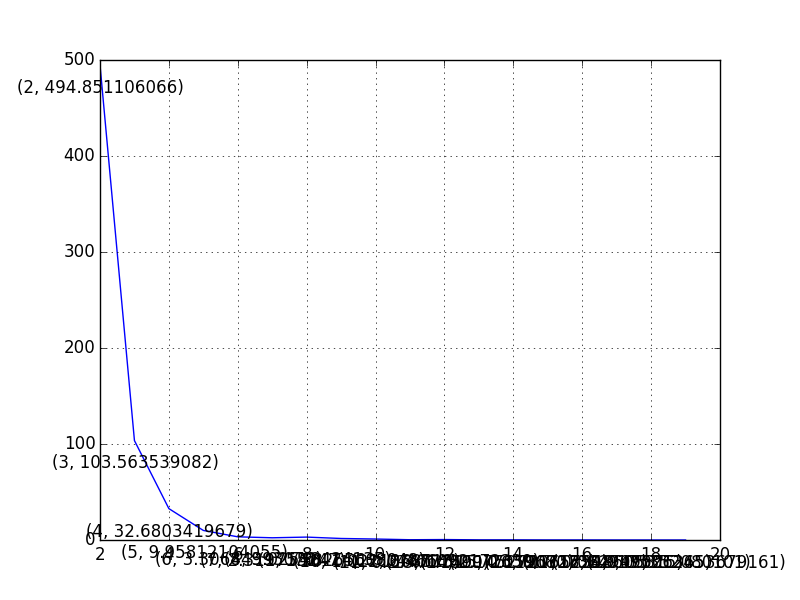
\includegraphics[width=2.8in]{figure/sscluster.png}
    \caption{Dendrogram for clustering after using sscluster}
    \label{sscluster}
\end{figure}
\begin{figure}
    \centering
    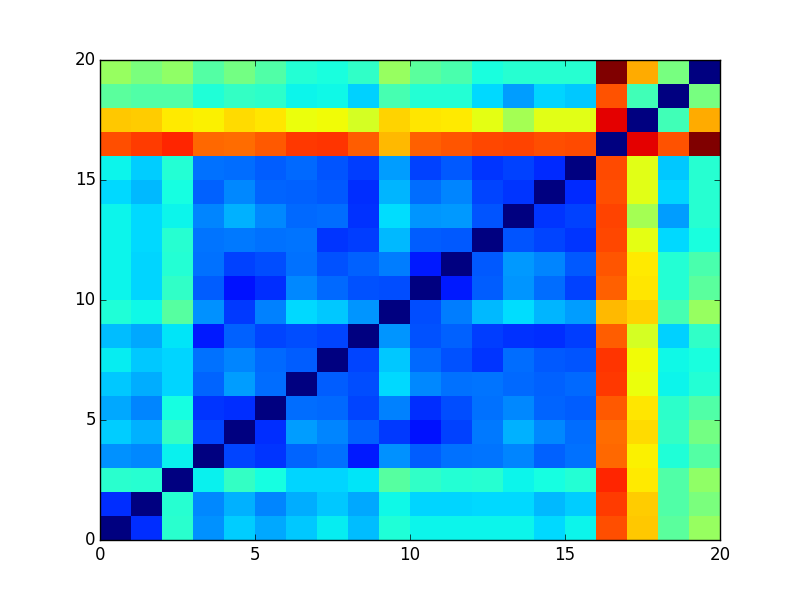
\includegraphics[width=2.8in]{figure/distance.png}
    \caption{Distance matrix for channels within one athlete}
    \label{athelet_distance}
\end{figure}
\begin{figure}
    \centering
    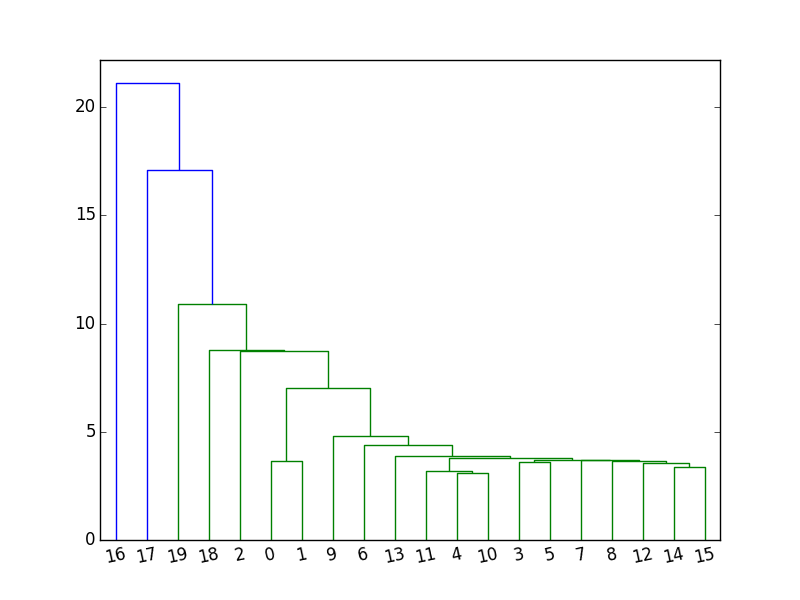
\includegraphics[width=2.8in]{figure/single1.png}
    \caption{Dendrogram of channels for one athelete}
    \label{athelet_dendrogram1}
\end{figure}
\begin{figure}
    \centering
    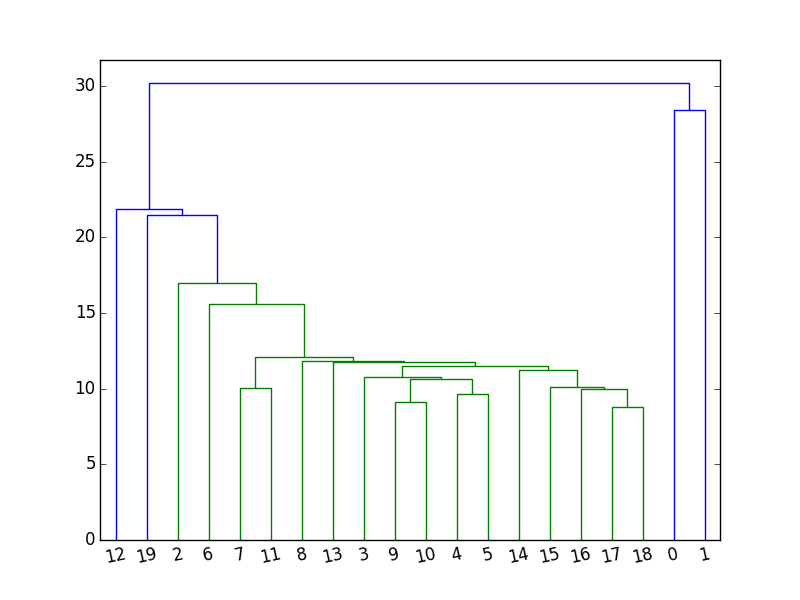
\includegraphics[width=2.8in]{figure/single2.png}
    \caption{Dendrogram of channels for another athelete}
    \label{athelet_dendrogram2}
\end{figure}
\begin{figure}
    \centering
    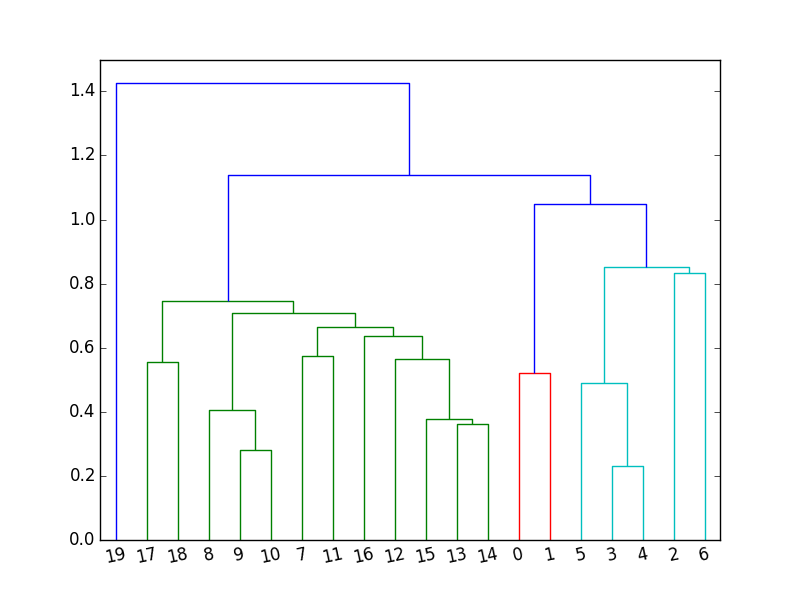
\includegraphics[width=2.8in]{figure/all1.png}
    \caption{Dendrogram of channels across athelete using 60 as time window, 10 as rolling window interval}
    \label{allathelet_dendrogram1}
\end{figure}
\begin{figure}
    \centering
    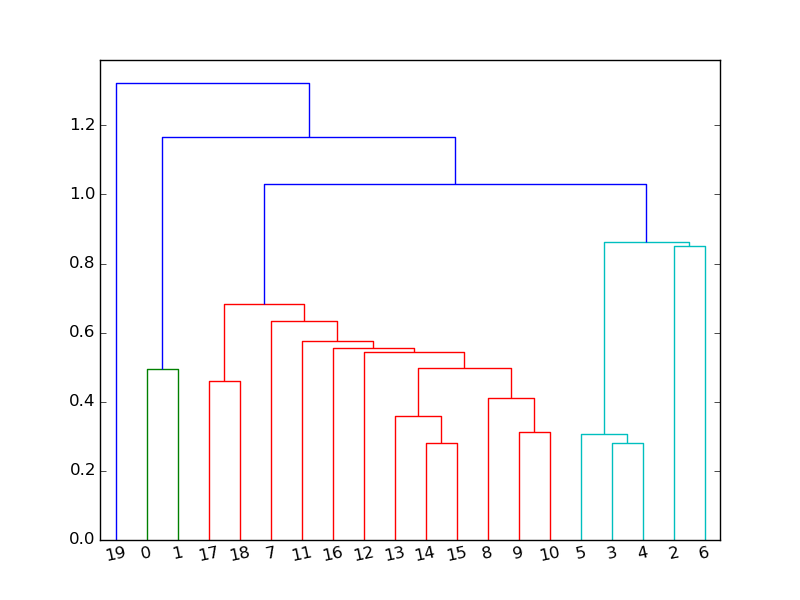
\includegraphics[width=2.8in]{figure/all2.png}
    \caption{Dendrogram of channels across athelete using 60 as time window, 15 as rolling window interval}
    \label{allathelet_dendrogram2}
\end{figure}